\documentclass[letterpaper]{article}
%% Language and font encodings
\usepackage[english]{babel}
\usepackage[utf8x]{inputenc}
\usepackage[T1]{fontenc}

%% Sets page size and margins
\usepackage[a4paper,top=3cm,bottom=2cm,left=3cm,right=3cm,marginparwidth=1.75cm]{geometry}
\errorcontextlines 10000
%% Useful packages
\usepackage{multirow}
\usepackage{amsmath}
\usepackage{graphicx}
\usepackage[colorinlistoftodos]{todonotes}
\usepackage[colorlinks=true, allcolors=blue]{hyperref}
\usepackage{tabularx}
\usepackage{natbib}
\usepackage{booktabs}
\bibliographystyle{plainnat}

\title{Prelim paper - Exploring transparency mechanisms to IDENTIFY failures}
\author{preetir }
\date{November 2018}

\usepackage{natbib}
\usepackage{graphicx}

\begin{document}

\maketitle

\section{Introduction}

\section{Flow}
Maybe start with Instructable robot - describe the robot's capabilities, then talk about failure situations 
\section{Related Work}
How do I compare with other related work? What are dimensions across which I can do that? (Refer to thesis intent part 1 to figure this out)

\section{Instructable Robot}
We have rosie who can do blah and blah.
In order to effectively teach the robot, the instructor needs a good model of what the robot already knows about the task and its environment. This includes the meaning of specific words that the robot understands and the objects and relations it can observe in its environment. However, the learned structures in the robot can not be accessed or modified by an instructor directly. This is because the internal form of these structures is optimized for task learning and execution, not explanation. Currently, only developers have interacted with this robot and they have a perfect model of what the robot can understand or its task, as well as, what it has learned in its past. In order for non-expert users to be able to teach these robots, they need to at least begin to understand the robot's point of view in terms of common knowledge and its environment.

Figure (teaching process) depicts an expert interaction where Rosie is being taught the task of Tower of Hanoi. The instructor begins teaching by providing the name of the puzzle they would like to teach. The agent drives the conversation by requesting specific information to help it learn the task. Based on a previous study, we realized that the teaching in Rosie is modular i.e. different components of Rosie can be taught individually to then compose a completely put together task. Each component teaching interaction starts off with an instructor defining a specific component, for example, in the figure, the instructor defines an action by saying ``You can move a clear block onto a clear object that is larger than the block''. In response to a component defining instruction, if it consists of concepts that the agent is not familiar with,then the agent asks the instructor for definitions of the same. In this example, the agent asks the instructor to define \emph{clear} and \emph{larger} since it does not know the meaning of either of these concepts. If the agent has completely interpreted and understood the instruction, the agent asks the instructor to set up the corresponding state in order for the agent to be able to imagine the action in its working memory. Once it has completely understood the instruction, the agent responds with an update that it has indeed learned the component and is ready for a new instruction. 

However, even with other humans, we do not have perfect communication. There are often misunderstandings, which arise on account of not being on the exact same understanding of any given situation and misconstruing existing language. These misunderstandings are then resolved by back and forth communication where both parties present relevant information in order to resolve this misunderstanding. We cannot expect a robot with limited interaction capabilities to be able to make sense of the human's misunderstanding and communicate the appropriate information, we need to rely on the human to be able to request the information that would potentially help them move further. Secondly, even if the user is an expert user who can use the right language, when exploring new capabilities, it is possible that they would like to understand what went wrong without having to debug the robot. Given these situations, it seems like the first step is for the user to have access to the robot's knowledge that contributes to their mental model of the robot, as a way to resolve this common ground. So our first step was to identify and characterize the types of knowledge that are present in the robot that would prove useful in a task teaching context. We then implemented different ways of accessing this knowledge that we discuss in later sections. We believe that that the robot knowledge being transparent to its users is a crucial first step to accomplishing common ground with the user.

\section{Characterization of robot knowledge}
\subsection{Perception}
Perception refers to the internal model of the environment that the robot dynamically builds up using its observations of the environment \textcolor{red}{potentially consider referrign to paper that does this}. Figure 1(tower of hanoi goal - show it in similar environment) shows the robot's interpretation of its environment. It is able to extract unary features of objects (including size, shape, color) and relations (such as that an object is ``on'' another object). In this formulation of Tower of Hanoi, the robot is able to recognize that there are in total six objects. It is able to identify that objects 4-6 represent locations and objects 1-3 represents blocks. It is able to identify the colors of these individual objects (green,blue) and is able to assign them sizes (small, medium) based on its previous training. Access to the robot's perception allows the instructor to verify that the robot has learned the appropriate perceptual classifiers and additionally, helps the instructor resolve common ground about the robot's labels of objects in their shared environment.

\subsection{Long-Term Task Knowledge}
As we referred before, the robot is capable of learning tasks from scratch using primitive knowledge alone. Learning a task comprises different aspects of the given task including goal definitions, actions, failure conditions and task predicates. Through natural language coupled with demonstration, the agent learns hierarchical representations of task components, that are first created in the working memory, and then stored for future use in the long term semantic memory. These concepts are depicted in the 

\subsection{Instantiating Task Knowledge}
In order for the agent to perform a task in its environment, it needs to be able to combine the former two types of knowledge - it must be able to apply its learned task knowledge in its environment. 
\begin{figure}
\centering
\frame{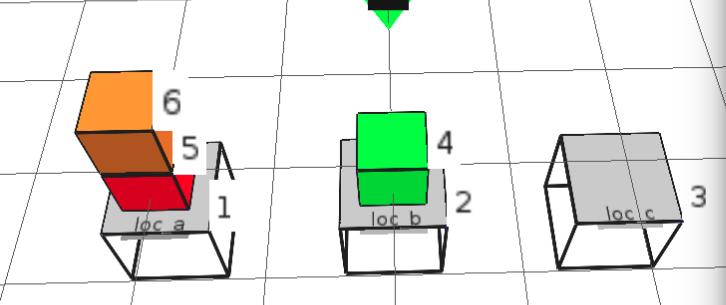
\includegraphics[width=\columnwidth]{blocks_world.png}}
 \caption{When the mentor is trying to describe the goal, they would say the following: ``The goal is that the red block is below an orange block and the red block is on a green block.'' to which the robot would respond with ``I do not see the goal.'' since the red block is not on the green block as described by the mentor.}
 \label{fig:blocks-goal}
\end{figure}
\section{Failure situations}
\textcolor{blue}{Now that we have discussed important knowledge for the user to access about the robot, we need to talk about situations where this knowledge and its presentation becomes even mroe relevant - failure situations. In order for the misunderstanding to be resolved, the user needs to be able to understand exactly why the robot failed. What kind of failures do we see occurring with the robot?}

These failure situations are represented by an environment setup for a particular game, along with a mentor instruction that has not been understood by the robot. For example, in figure \ref{fig:blocks-goal}, the mentor wants the robot to learn the goal of Blocks World namely, ``The goal is that the red block is below an orange block and the red block is on a green block.'' and a situation is presented in the shared environment. However, it can be observed that the goal is not present in the environment, since one of the conditions, the red block on the green block, is not satisfied. The implemented language mechanisms enables the robot to specify that it cannot see the goal because ``the red block is not on the green block''.

\begin{figure}[ht!]
\centering
\frame{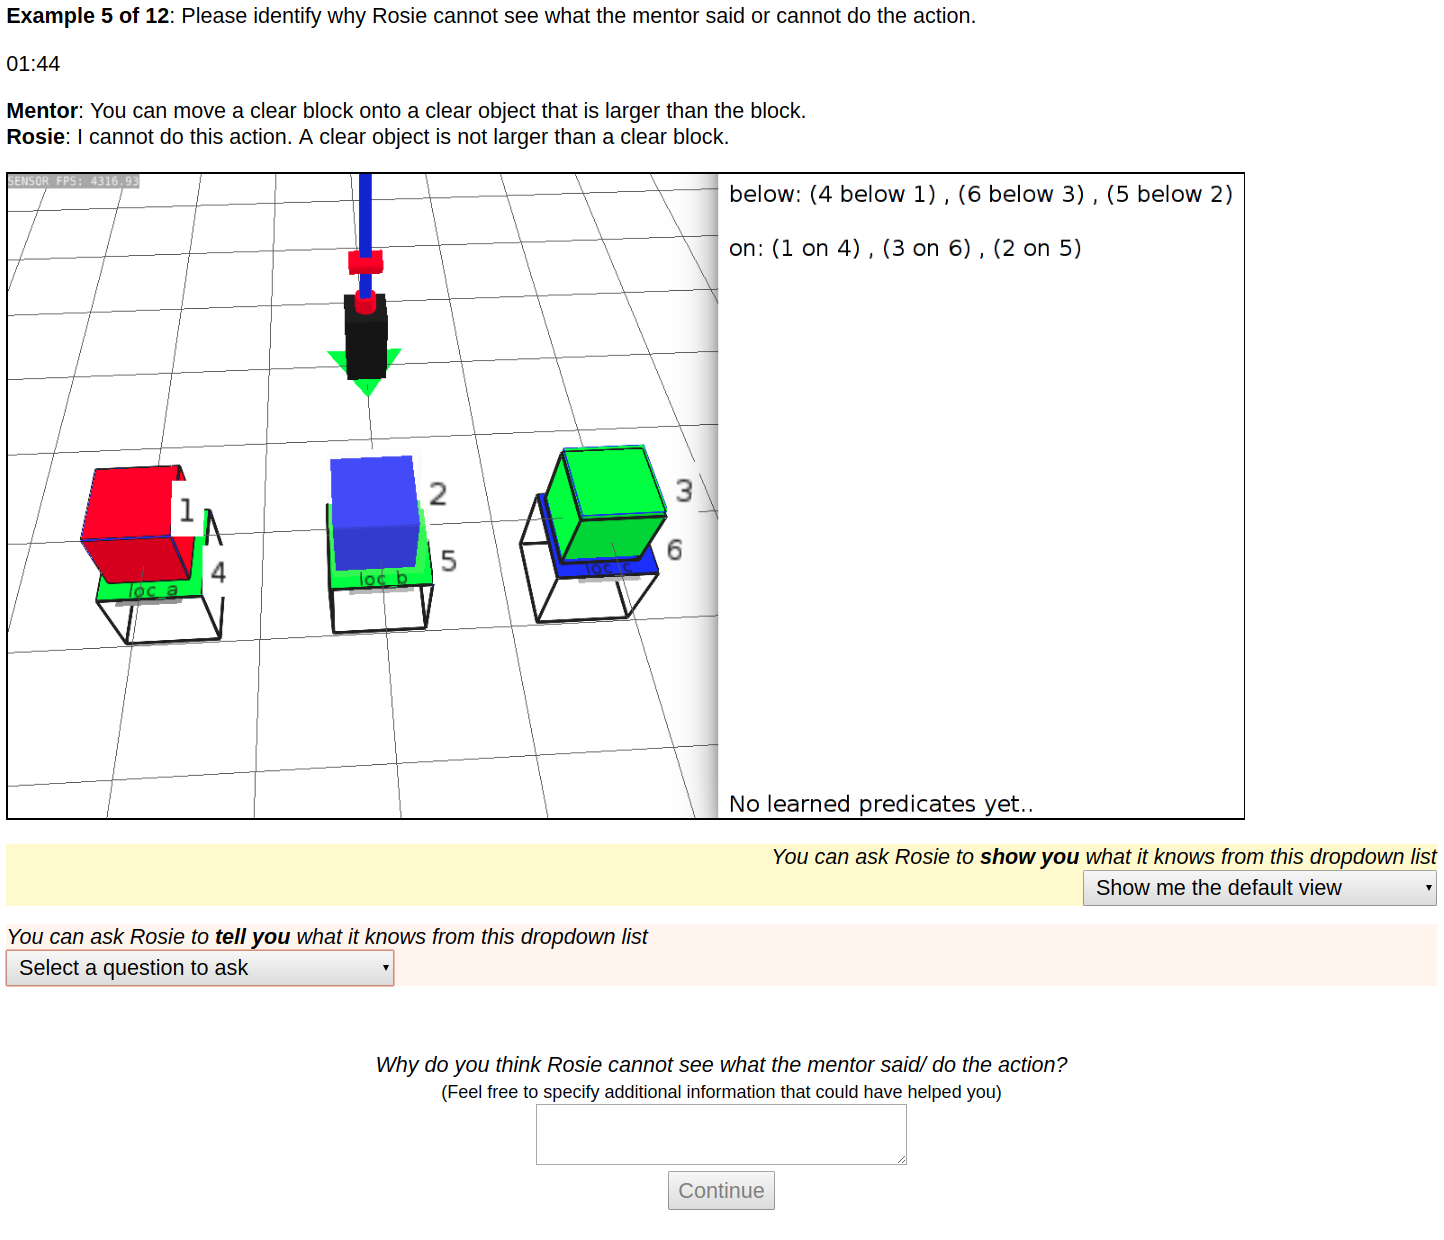
\includegraphics[width=\columnwidth]{user_study_interface.png}}
\caption{Mechanical turk user interface presented to the user}
\label{fig:user-interface}
\end{figure}

\section{Implementation}
However, we are currently assuming that the robot does not have enough knowledge to be able to use context cues and previous conversations, in order to provide the exact information during failure. So assuming that the user has control over this conversation and would like to 
\section{User Study}
\textcolor{red}{be explicit that you have replicated potential interaction with robot. yes you are losing out by not having real-time interaction but as a compromise, you get to evaluate the information providing mechanisms of the same on a quantitative level. specify how you came up with 3 minute timeline/. You don't need to necessarily test it out on a real robot BUT you need to be able to give me a convincing point of view that if this is put on a robot it will run}
We conducted this study on Mechanical Turk [refer Walter's paper]. We presented each user with 12 failure situations spanning across five different games and puzzles that the robot has encountered in the past. The goal of the user is to identify the failure using the transparency mechanisms that are available with each situation. The games and puzzles include Tic-Tac-Toe, Tower of Hanoi, Blocks World, Nine Holes and Simple Maze. 

Each user got access to 12 failure situations, 4 of each difficulty level (easy, medium, and difficult), and 3 of each transparency level(None, Q-A, Visual Explanation, and Both Q-A and Visual Explanation) which we will describe below. Figure \ref{fig:user-interface} shows the interface of a specific example where both transparency mechanisms are made available to the user. In this case, the mentor is describing what they expect the robot to see in the environment, and the robot responds with its understanding of the same environment.
\begin{quote}
Mentor: Three locations in a line are captured.
\textit{Rosie: I do not see that. Three locations in a line are not captured.}
\end{quote}

As can be observed in Figure \ref{fig:user-interface}, the user can either ask Rosie to \emph{tell them} or \emph{show them} what it knows in terms of previous learned knowledge and its environment. The questions list consists of all the questions that the robot is capable of answering right now and similarly, the visual explanation list consists of mechanisms through which the user can see the properties and relations of the objects in the environment as well as the robot's understanding of previously learned predicates and situating it in its environment. For example, here the user can ask the question ``What is captured?'' in order to then learn that the robot defines it as follows: ``If an object is below a red block , then it is captured.'' Instead, the user could also ask the robot to show which objects are captured, at which point the robot will highlight objects 1 and 4 to indicate that they are captured. The user could also ask ``Which locations are in a line?'', in order to get a list of locations that are in a line according to the robot, in order to then identify the failure in the situation. Similarly, the user can verify the robot's thoughts of which objects are in a line through the side panel presented next to the situation image. 

Now that the user understands that only two locations are \emph{captured}, hence the robot does not see what the mentor expects it to see, we ask the user to provide two inputs about their thoughts. First, we ask them to describe in their own words, why Rosie cannot confirm the environment description or do the action as was expected by the mentor. Once they write their understanding of the situation and press the ``Continue'' button, the text box disappears (since they are not allowed to change their input) and they are provided with a multiple-choice drop-down list of answers from among which they are asked to select the right one. There is only one correct answer per question. The user is also asked to provide their confidence in their selected answer on a Likert scale of range 1-5. We recorded the time taken per example for each user at every time instant.

Even though the mechanical turk environment did not provide access to the robot in itself, the various projections of the environment, the visual and question-answering capabilities equivalently replicated what is currently possible in the robot. Our goal here was to evaluate the mechanisms for the information that they share, the manner in which they are shared, and their contribution to the user's mental model of the robot. Keeping that in mind, we designed the study to be a less dynamic version of what is capable in the robot.

Even though all the 12 failure situations presented to all the users were exactly the same, the transparency mechanisms linked to each example was differed randomly by the user. In that sense, this study was both a within and between subjects study - We study the effects of varying transparency mechanisms within the different examples that the user is presented with and we also get the effects of varying transparency mechanisms on the same example across different users.

The four transparency mechanisms are described as follows:
\begin{enumerate}
    \item None: I
    \item QnA: The questions included things about its perception, its knowledge. For example, in this example, the user will be able to ask ``What is on the location 5' about all locations, ``What is below the block 3'' about all the blocks, they can ask to describe every object in the environment and this description would include the features of the objects as well as its individual relations. Additionally, if the mentor's description included a learned predicate that has a special meaning, which is ``captured'' here, the questions also include being able to ask a definition of ``captured'' so that the user can then use the description.
\end{enumerate}

\section{Data Analysis}
Describe more clearly how you analyzed the accuracy data. I think the confidence and time data were adequately described.
\section{things that could be better(better title)}
the questions were fairly limited. it would have been better if the person could ask the questions they found relevant and if we had answers for that or not. for e.g. instead of asking "describe blue block" and getting all possible near and diagonal relations, all i needed to ask was "is blue block adjacent to location 3?", and be told "no" and then when someone asks why, maybe break down the definition of adjacent to say "because it is not near"
We definitely agree that a person being able to ask free-form questions/visual actions would be more reflective of a real conversation, and that interaction with a real robot would bring in new perspectives and that's something we would like to explore in the future. 

\section{Conclusion}
``I always thought something was fundamentally wrong with the universe'' \citep{adams1995hitchhiker}
\bibliographystyle{plain}
\bibliography{references}
\end{document}
